\chapter{まとめ}

\section{本論文のまとめ}
HL-LHCに向けてATLAS内部飛跡検出器の総入れ替えを予定しており、これに向けてピクセルモジュールを世界で約10,000台生産する予定である。
各モジュールに対して品質試験を行い、全てのモジュール及び品質試験の結果は中央データベースに保存する。

本研究では、この生産及び品質試験に向けてデータベースシステムの構築を行った。
各組み立て機関にてデータ管理をするローカルデータベースを確立し、品質試験結果検索や中央データベースとの同期機能など、生産時に必要となる諸ツールの開発を行った。

開発した諸ツールを含め、生産において必要な機能の確認を行った。本番を想定したソフトウェア、ハードウェアのセットアップと各ツールの処理を実行し、機能が使用可能であることを確認した。

主な開発項目の1つ目として品質試験検索機能を述べた。
開発当初はデータベース内部構造により試験結果数$n$に対して処理時間が$O(n^2)$となり、運用時における見積もりが$(9.8±0)\times 10^3$[sec]となってしまい、実用に向かない機能であった。
MongoDB内に新しいコレクションを設け検索に必要な情報を予めドキュメントに保持しておくことにより、処理時間の改善に成功した。
実際に処理時間の測定を行い、データ数の増加に対しても検索機能が不都合なく使えることを確認した。
本番を想定した見積もりを行い、84,000件のデータ数に対して$2.6\pm0.1$[sec]で処理が実行できる見込みであり、生産時において有用な機能であることを確認した。

2つ目に中央データベースとローカルデータベースの同期ツールを開発した。
世界的に使われるツールであり、全ての組み立て機関でこのツールをサポートするために中央データベースへの通信処理時間調査をKEK、LBNL、CERNのサーバーを用いて行った。
KEKのサーバーを用いた場合に最も時間がかかることを確認した。

同期ツールに関して、モジュール情報のダウンロード、読み出し試験結果のアップロード機能を開発した。
モジュール情報のダウンロード機能に関して、KEKサーバーを用いてその処理時間測定を行い、Quadモジュール1つあたり$4.0\pm 0.4$[sec]の処理時間がかかることを確認した。
処理の詳細を調査すると、モジュールや構成部品の情報取得するために行っている中央データベースAPIの使用に時間がかかっていた。
処理時間の改善策をいくつか考案し、それぞれについて見積もりを行った。
読み出し試験結果のアップロード機能に関して、開発当初は読み出し試験結果5項目のアップロードにおける処理時間の見積もり値が$7.9 ± 0.1$[min]であった。
処理時間改善に向けて処理の詳細を調査したところ、結果ファイルの添付処理に大きく時間が要していることが分かった。
ファイル添付についての詳細を調べると、添付処理時間がファイル数とファイル容量に依存していた。
このことから結果ファイルをZIPファイルにまとめ、圧縮しアップロードを行うことで処理時間の改善を図った。
ここで圧縮前後のファイル容量は、それぞれ94、3.9[MB/FEチップ]となった。
結果として処理時間の改善に成功し、その見積もり値が$1.2\pm 0.1$[min]となった。

\section{現状と今後の課題}
\subsection{ソフトウェアリリースとユーザサポート}
本論文で述べたツールの他に、読み出し試験コマンド統括ソフト、品質試験結果アップロード用ソフトなどの開発もチームとして行っている。
全てのソフトウェアを含めて、品質試験のデータ管理を達成するようなアプリケーションスイートを目指している。
2020年12月9日にファーストバージョンのリリースを行い、いくつかの機関で全体のシステム及びソフトウェアが使われている現状である。

またCERNで行ったチュートリアルを経て、世界的に機能普及が進んでいる。
そのためユーザサポートとしてソフトウェア使用のためのドキュメント\cite{7-1}の作成、整備も行っている。
開発者の連絡先やローカルデータベース専用掲示板へのリンクもドキュメントに記している。何か問題が生じた時などに簡単に問い合わせができる仕組みを整えている。

\subsection{開発課題}
本研究では検索機能や同期機能など、読み出し試験を対象とした機能を重点的に開発した。
ローカルデータベース開発は、読み出し試験の結果を管理したいという要求から始まり、現在はそれ以外の品質試験も含め、全ての試験結果や組み立て工程の管理も目標としている。
今後の開発課題として以下の機能をあげる。
\begin{itemize}
  \item 読み出し試験以外(外観検査、平坦性測定等)の結果同期機能.
  \item 中央データベースからローカルデータベースへ品質試験結果の同期.
  \item 品質試験結果解析とモジュール選別機能. 
  \item 組み立て工程管理を世界的にサポート.
\end{itemize}

最後の項目に関して、モジュールの組み立て工程は各機関ごとに異なるため、全ての現場における工程を調査しそれをサポートするシステムを実装する必要がある。
例えば、日本では「ベアモジュール・フレキシブル基板貼り付け」工程の後に、モジュール冷却のための構造である「セル搭載」を行う予定であり、これは他の組み立て機関とは異なる。
各地域における柔軟な生産を許しているため、組み立て工程は世界的に細かく統一されていない。
データベースシステムでは多様な組み立て工程に対応できるシステムとする必要がある。

柔軟な組み立て工程のサポートに向けて、中央データベースには選択可能な組み立て工程を定義する機能が存在し、これを使用することを考えている。
そのイメージを図\ref{optional_stage}に示す。

\begin{figure}[bpt]\centering
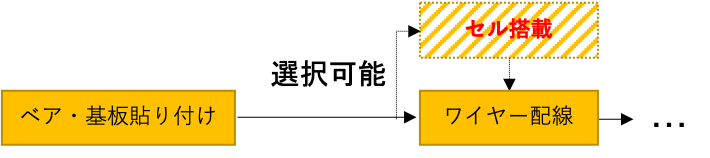
\includegraphics[width=10cm]{./optional_stage.png}
\caption[中央データベースにおける選択可能な組み立て工程のイメージ]{中央データベースにおける選択可能な組み立て工程のイメージ。図に示すように中央データベースでは選択可能な組み立て工程を定義することができる。図ではセル搭載が選択可能となっていて、ベア・基板貼り付け工程の後に、どちらの工程に進むのかを選択できる。この機能を用いて世界的に多様な組み立て工程をサポートすることを考えている。}
\label{optional_stage}
\end{figure}

以下の開発項目をあげる。
\begin{itemize}
  \item 中央データベースにおいて選択可能な工程定義機能を使い、全ての組み立て機関における工程をサポートする構造を設計、実装.
  \item 本研究で開発した同期ツールを拡張、ローカルデータベース上にも中央データベースと同様の組み立て工程構造を保持.
\end{itemize}

これらを達成することにより、全ての機関における組み立て工程情報の管理ができるようになると考えている。


